%\documentclass{article}
%\usepackage{graphicx,subfigure}
%\begin{document}

\begin{figure}[!h]
  \centering
  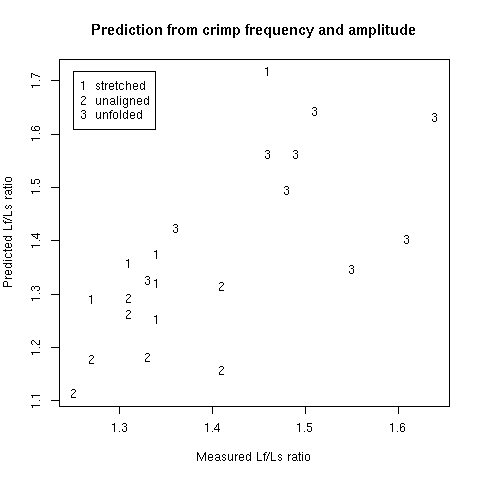
\includegraphics[width=1.0\textwidth]{figpfarat.png}
%   predratf.png is original 
  \caption{Plot of measured fibre length to staple length ratio against predicted fibre length to staple length ratio. Predictions calculated from crimp frequency and amplitude.}
  \label{fig:pfarat}
\end{figure}

%\end{document}

